\chapter{ការបង្កើតផេកតាមស្តង់ដារ និងការ}
\quad\quad ការធ្វើអាជីវកម្មតាមយុគសម័យថ្មី គឺពឹងផ្អែកលើវិស័យបច្ចេកវិទ្យាដើម្បីផ្សព្វផ្សាយ ផលិតផលរបស់យើងឱ្យទៅដល់អថិតិជនចំគោលដៅ។ 
\section{ការបង្កើតផេកតាមកុំព្យូទ័រ}
\quad\quad ជាដំបូងខ្ញុំ សូមធ្វើការបង្ហាញការបង្កើតផេកឬហៅថាទំព័រហ្វេសប៊ុកនៅលើ កុំព្យូទ័រ។ សូមធ្វើការចុច​លើសញ្ញា ព្រួញចុះក្រោម រួចចុចយកពាក្យ {\en (Manage Pages)}។ 
\subsection{របៀបដាក់ឈ្មោះផេកហ្វេសប៊ុក}
\begin{enumerate}
	\item ចុចលើសញ្ញា ព្រួញចុះក្រោម
	\item ចុចយកពាក្យ {\en Manage Page}
	\item ចុចយកពាក្យ​ {\en Create a Page}
	\begin{figure}[H]
		\centering
		\begin{tikzpicture}
		\node at (0,0) {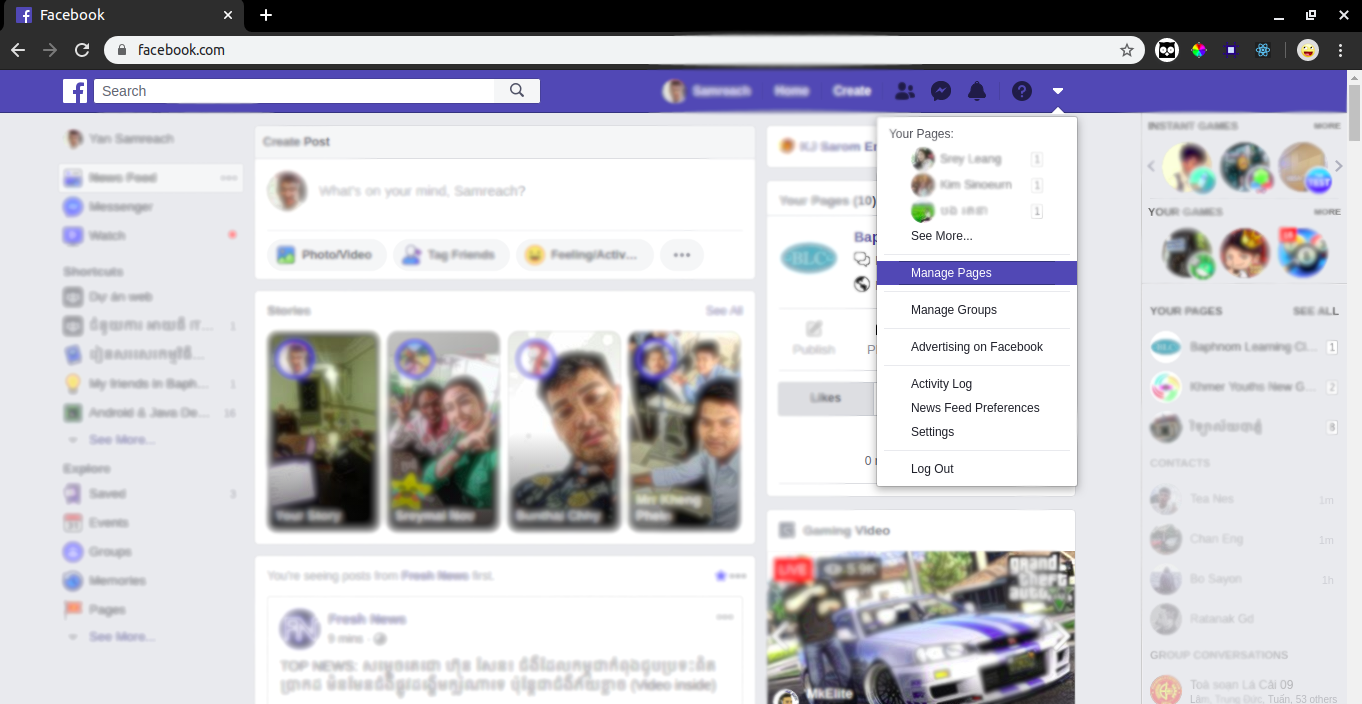
\includegraphics[scale=.4]{page1}};
		\end{tikzpicture}
	\end{figure}
\end{enumerate}